\chapter{Materials and Methods}
\label{ch:methods}

\section{Robot platform}
\label{sec:platform}

A Waveshare RaspRover with a Raspberry Pi~5 was used~\citep{waveshare_rasprover}. Instead of rebuilding the chassis from the previous work~\citep{graham2024}, this platform was chosen because it already has four driven wheels with encoders, an inertial measurement unit (IMU), a voltage measurement and its own motor controller. A Slamtec RPLIDAR A2M12 lidar was used to sense the environment~\citep{slamtec_a2m12}.

The robot has two controllers (Fig.~\ref{fig:architecture}). The Raspberry Pi~5 is the main computer and runs ROS2 and all other software. An ESP32 microcontroller on the Waveshare driver board controls the motors and reads the sensors on the board~\citep{waveshare_driver}. The Raspberry Pi is plugged onto the driver board with its 40-pin header, which provides both the \SI{5}{\volt} supply and the UART connection to the ESP32. Table~\ref{tab:components} lists the sensors and actuators.

\begin{figure}[H]
  \centering
  \begin{tikzpicture}[
      font=\small,
      box/.style={draw, rounded corners=2pt, align=center, minimum height=1cm, inner sep=5pt, fill=white},
      comp/.style={box, minimum width=2.6cm},
      arr/.style={-{Stealth[length=2mm]}, thick},
      lbl/.style={font=\scriptsize, fill=white, inner sep=1pt}
    ]
    \node[comp, minimum width=4.0cm, minimum height=1.6cm] (pi) {\textbf{Raspberry Pi 5}\\ROS2 Jazzy (Docker)\\bridge node};
    \node[comp, minimum width=4.0cm, minimum height=1.6cm, right=2.6cm of pi] (esp) {\textbf{ESP32}\\(driver board)\\PID motor control};
    \node[comp, above left=1.0cm and -1.6cm of pi] (lidar) {RPLIDAR A2M12};
    \node[comp, above right=1.0cm and -1.6cm of pi] (cam) {USB camera\\5\,MP, 160°};
    \node[comp, above left=1.0cm and -1.6cm of esp] (imu) {9-axis IMU};
    \node[comp, above right=1.0cm and -1.6cm of esp] (ina) {INA219\\voltage};
    \node[comp, below left=1.0cm and -1.6cm of esp] (mot) {4$\times$ N20 motor\\with encoder};
    \node[comp, below right=1.0cm and -1.6cm of esp] (oled) {OLED, LEDs};
    \node[comp, minimum width=2.1cm, right=0.8cm of esp] (bat) {3S battery\\UPS module};
    \draw[arr, <->] (pi) -- node[lbl, above] {UART (JSON)} node[lbl, below, align=center] {40-pin header\\+ \SI{5}{\volt} supply} (esp);
    \draw[arr] (lidar) -- node[lbl, left] {USB / UART} (pi);
    \draw[arr] (cam) -- node[lbl, right] {USB} (pi);
    \draw[arr] (imu) -- node[lbl, left] {I\textsuperscript{2}C} (esp);
    \draw[arr] (ina) -- node[lbl, right] {I\textsuperscript{2}C} (esp);
    \draw[arr, <->] (esp) -- node[lbl, left] {PWM / enc.} (mot);
    \draw[arr] (esp) -- node[lbl, right] {I\textsuperscript{2}C / PWM} (oled);
    \draw[arr, dashed] (bat) -- node[lbl, above] {power} (esp);
  \end{tikzpicture}
  \caption{Hardware architecture of the robot.}
  \label{fig:architecture}
\end{figure}


\begin{table}[H]
  \centering
  \small
  \caption{Sensors and actuators of the robot.}
  \label{tab:components}
  \begin{tabularx}{\textwidth}{@{}l l l X@{}}
    \toprule
    \textbf{Type} & \textbf{Component} & \textbf{Interface} & \textbf{Data / function} \\
    \midrule
    Sensor   & RPLIDAR A2M12             & UART over USB   & 360° 2D scan~\citep{slamtec_a2m12} \\
    Sensor   & Wheel encoders            & ESP32           & Speed and distance of each side \\
    Sensor   & 9-axis IMU                & I\textsuperscript{2}C, ESP32 & Acceleration, angular rate and magnetic field~\citep{waveshare_driver} \\
    Sensor   & INA219                    & I\textsuperscript{2}C, ESP32 & Battery voltage~\citep{waveshare_driver} \\
    Sensor   & USB camera                & USB             & Not used in this work \\
    Actuator & 4 DC gear motors          & ESP32           & Drive (skid steering) \\
    Actuator & Lidar motor               & Lidar           & Rotation of the lidar head \\
    \bottomrule
  \end{tabularx}
\end{table}

The robot is powered by three 18650 lithium-ion cells (3S) with a UPS module, so it can be charged while it is running~\citep{waveshare_rasprover}.

\section{Software environment}
\label{sec:software}

The Raspberry Pi runs the Raspberry Pi OS image from Waveshare (Debian Bookworm, 64-bit), which includes a web application for remote control. This web application blocks the serial port to the ESP32, so its autostart entry in \texttt{crontab} was disabled.

ROS2 Jazzy Jalisco was chosen because it is a long-term support (LTS) release~\citep{ros2_jazzy}. This also follows the recommendation of the previous work to use an LTS release instead of Rolling~\citep{graham2024}. ROS2 Jazzy is made for Ubuntu~24.04 and not for Raspberry Pi OS. Therefore, ROS2 was run in a Docker container based on the official image \texttt{ros:jazzy-ros-base}. This way, the manufacturer image stays unchanged. The container was started with host networking (for the visualisation on the laptop), with access to the device files (serial port of the ESP32 and the lidar) and with the ROS2 workspace mounted from the Raspberry Pi, so the code is not lost when the container is deleted (Appendix~\ref{app:code}).

\section{Communication with the ESP32}
\label{sec:protocol}

The Raspberry Pi communicates with the ESP32 over UART (\texttt{/dev/ttyAMA0}, \SI{115200}{baud}). Each message is one line of JSON, and the key \texttt{T} gives the command type~\citep{waveshare_json}. The following commands were used (overview in Appendix~\ref{app:commands}):

\begin{itemize}
  \item \texttt{\{"T":900,"main":1,"module":0\}} sets the chassis type to RaspRover. This has to be sent after every start, otherwise the direction and speed of the wheels are wrong.
  \item \texttt{\{"T":13,"X":$v$,"Z":$\omega$\}} sets the linear velocity $v$ in \si{\metre\per\second} and the angular velocity $\omega$ in \si{\radian\per\second}.
  \item \texttt{\{"T":131,"cmd":1\}} switches on the continuous feedback.
\end{itemize}

The firmware has a heartbeat function, which stops the motors when no new drive command arrives for some time~\citep{waveshare_json}. With continuous feedback switched on, the ESP32 sends a feedback message (\texttt{"T":1001}) with wheel speeds, distance counters, raw IMU values and the battery voltage (example in Appendix~\ref{app:rawdata}). The units of these values are not documented, so they had to be determined with tests (Section~\ref{sec:calibration_method}).

\section{ROS2 bridge node}
\label{sec:bridge}

Waveshare does not provide a ROS2 driver for the robot. Therefore, a bridge node (\texttt{rasprover\_bridge}) was written in Python (Fig.~\ref{fig:bridge}, code in Appendix~\ref{app:code}). It translates between the standard ROS2 topics and the JSON commands of the ESP32, so that standard packages like SLAM Toolbox and Nav2 can use the robot.

\begin{figure}[H]
  \centering
  \begin{tikzpicture}[
      font=\small,
      box/.style={draw, rounded corners=2pt, align=center, minimum height=0.9cm, inner sep=5pt, fill=white},
      arr/.style={-{Stealth[length=2mm]}, thick},
      lbl/.style={font=\scriptsize, fill=white, inner sep=1pt}
    ]
    \node[box, minimum width=3.0cm] (cmd) {\texttt{/cmd\_vel}};
    \node[box, minimum width=3.0cm, below=0.35cm of cmd] (odom) {\texttt{/odom}, TF};
    \node[box, minimum width=3.0cm, below=0.35cm of odom] (imu) {\texttt{/imu/data\_raw}};
    \node[box, minimum width=3.0cm, below=0.35cm of imu] (bat) {\texttt{/battery\_state}};
    \node[box, right=1.3cm of cmd, minimum width=3.4cm] (timer) {send timer\\\SI{20}{\hertz}};
    \node[box, right=1.3cm of imu, minimum width=3.4cm, yshift=0.65cm, minimum height=2.2cm] (reader) {read thread\\parse JSON\\convert units\\integrate odometry};
    \node[box, right=2.3cm of timer, minimum width=2.0cm, minimum height=4.6cm, yshift=-1.95cm] (esp) {\textbf{ESP32}};
    \begin{scope}[on background layer]
      \node[draw, dashed, rounded corners, fit=(timer)(reader), inner sep=8pt, label={[font=\scriptsize]above:\texttt{rasprover\_bridge}}] {};
    \end{scope}
    \draw[arr] (cmd) -- (timer);
    \draw[arr] (timer) -- node[lbl, above=2pt] {\texttt{\{"T":13,...\}}} (timer -| esp.west);
    \draw[arr] (reader -| esp.west) -- node[lbl, above=2pt] {\texttt{\{"T":1001,...\}}} (reader);
    \draw[arr] (reader.west) -- ++(-0.6,0) |- (odom);
    \draw[arr] (reader.west) -- ++(-0.6,0) |- (imu);
    \draw[arr] (reader.west) -- ++(-0.6,0) |- (bat);
  \end{tikzpicture}
  \caption{Structure of the bridge node.}
  \label{fig:bridge}
\end{figure}


\paragraph{Structure.} A timer sends the current drive command to the ESP32 every \SI{50}{\milli\second}. A separate thread continuously reads the serial port and processes every feedback message. A lock makes sure that two commands are not written at the same time.

\paragraph{Start.} At the start, the node sets the chassis type and switches on the feedback. The robot then has to stand still for \SI{2}{\second} while the node averages the gyroscope values to get the offset $b$. During this time, no drive commands are sent.

\paragraph{Commands.} The node takes the linear velocity $v$ and the angular velocity $\omega$ from \texttt{/cmd\_vel} and sends them as a \texttt{T:13} command. The ESP32 converts them to wheel speeds. If no message arrives for \SI{0.5}{\second}, the node sends a stop command. Together with the heartbeat of the ESP32, the robot therefore stops if either the program sending the commands or the bridge node itself crashes.

\paragraph{Odometry.} Each feedback message is converted to SI units (Tab.~\ref{tab:feedback}). Because the robot slips a lot when it turns (Section~\ref{sec:calibration_results}), the distance is taken from the wheel encoders, but the heading is taken from the gyroscope. With the changes of the distance counters $\Delta n_l$ and $\Delta n_r$, the scale factor $s$, the angular rate $\omega_z$ (without offset) and the time step $\Delta t$:

\begin{align}
  d &= \tfrac{1}{2}\,s\,(\Delta n_l + \Delta n_r), \qquad \psi_k = \psi_{k-1} + \omega_z\,\Delta t, \\
  x_k &= x_{k-1} + d\,\cos\!\left(\psi_{k-1} + \tfrac{1}{2}\,\omega_z\,\Delta t\right), \qquad
  y_k = y_{k-1} + d\,\sin\!\left(\psi_{k-1} + \tfrac{1}{2}\,\omega_z\,\Delta t\right).
\end{align}

The distance counters are reset when the ESP32 restarts. Therefore, only the differences are used, and jumps of more than \SI{0.5}{\metre} between two messages are ignored.

\paragraph{Topics.} Table~\ref{tab:topics} shows the topics of the bridge node. The frames follow REP~103 and REP~105~\citep{rep103,rep105}. The conversion factors, the port, the command rate and the timeout are ROS2 parameters, so they can be changed without changing the code.

\begin{table}[H]
  \centering
  \small
  \caption{Topics of the bridge node.}
  \label{tab:topics}
  \begin{tabularx}{\textwidth}{@{}l l X@{}}
    \toprule
    \textbf{Topic} & \textbf{Message type} & \textbf{Content} \\
    \midrule
    \texttt{/cmd\_vel} (input) & \texttt{geometry\_msgs/Twist}       & Drive commands \\
    \texttt{/odom}             & \texttt{nav\_msgs/Odometry}         & Position and velocity from encoders and gyroscope \\
    \texttt{/tf}               & \texttt{odom} $\rightarrow$ \texttt{base\_link} & Position of the robot relative to its start position \\
    \texttt{/imu/data\_raw}    & \texttt{sensor\_msgs/Imu}           & Acceleration and angular rate \\
    \texttt{/battery\_state}   & \texttt{sensor\_msgs/BatteryState}  & Battery voltage and rough charge level \\
    \bottomrule
  \end{tabularx}
\end{table}

\section{Calibration of the sensor values}
\label{sec:calibration_method}

The units and scale factors of the feedback values were determined with simple tests on a smooth floor indoors. Distances were measured with a measuring tape, angles were estimated by eye. Because the ESP32 sends feedback continuously, the serial input buffer was cleared before each reading, so that the newest message was used.

\begin{itemize}
  \item \textbf{Wheel speed and distance:} The robot drove forward and backward with \SI{0.3}{\metre\per\second} for about \SI{3.3}{\second}. The values \texttt{L}/\texttt{R} and the changes of the counters \texttt{odl}/\texttt{odr} were recorded and compared with the measured distance.
  \item \textbf{Accelerometer:} The vertical acceleration was read while the robot was standing on a flat floor and while it was lying upside down.
  \item \textbf{Gyroscope offset:} The mean of 30 values of the vertical angular rate was calculated while the robot was standing still.
  \item \textbf{Gyroscope scale:} The robot turned on the spot for \SI{3}{\second} with a commanded angular velocity of \SI{1.5}{\radian\per\second}. The values (without offset) were integrated over time with the trapezoidal rule and divided by the estimated rotation angle.
\end{itemize}

\section{Test of the bridge node}
\label{sec:validation_method}

The rate of \texttt{/odom} was measured with \texttt{ros2 topic hz}. After that, the robot was driven manually with \texttt{teleop\_twist\_keyboard} (\SI{0.2}{\metre\per\second}, \SI{1.05}{\radian\per\second}) in two tests, and the position on \texttt{/odom} was recorded:

\begin{itemize}
  \item \textbf{Straight drive:} After restarting the node, the robot drove straight ahead for about \SI{1}{\metre}. The odometry was compared with the measured distance and the visible deviation from a straight line.
  \item \textbf{Turn:} The robot turned to the left on the spot by about \SI{90}{\degree}. The heading was calculated from the orientation quaternion as $\psi = 2\arcsin(q_z)$, which is valid for a rotation around the vertical axis only.
\end{itemize}

The drift of the heading while standing still was read from the recordings before and after the movements.

\section{Lidar integration}
\label{sec:lidar_method}

The lidar was connected to a USB port of the Raspberry Pi with the USB--UART adapter that comes with the sensor (\texttt{/dev/ttyUSB0}). The ROS2 driver \texttt{sllidar\_ros2} from Slamtec was built from source in the container and started with its launch file for the A2M12 (\SI{256000}{baud}). The driver publishes the scan on \texttt{/scan} (\texttt{sensor\_msgs/LaserScan}) in the frame \texttt{laser}.

The Raspberry Pi~5 limits the current of its USB ports when it is not powered by the official power supply. Because the Pi is powered by the driver board of the robot, this limit was switched off with the setting \texttt{usb\_max\_current\_enable=1} in \texttt{/boot/firmware/config.txt} (Section~\ref{sec:lidar_results}). Undervoltage was checked with \texttt{vcgencmd get\_throttled}.

The scan was checked with \texttt{ros2 topic hz} and by holding a hand at a known position in front of the lidar. For the visualisation, Foxglove was used, a tool for visualising robot data. The \texttt{foxglove\_bridge} runs as a node on the robot and provides the ROS2 topics over a WebSocket connection, so that the Foxglove application on another computer can display them and also publish messages~\citep{foxglove_bridge}. The scan was shown in the Foxglove desktop application on a laptop in the same network. For this first test, the lidar was just placed on the robot without fixing it.

\paragraph{Mounting.} To fix the lidar on the robot, an adapter plate was designed in FreeCAD and 3D-printed (Fig.~\ref{fig:mount}). The plate is $80 \times 65$\,mm and has eight holes with a diameter of \SI{3.3}{\milli\metre} for M3 screws. The holes are arranged in two square patterns of \SI{34}{\milli\metre} and \SI{42}{\milli\metre}, one for the lidar and one for the robot. The plate was printed several times and adjusted until both hole patterns fitted. \todo{Plate thickness, material and printer; which hole pattern is for the lidar and which for the robot.}

\begin{figure}[H]
  \centering
  \begin{subfigure}[b]{0.56\textwidth}
    \centering
    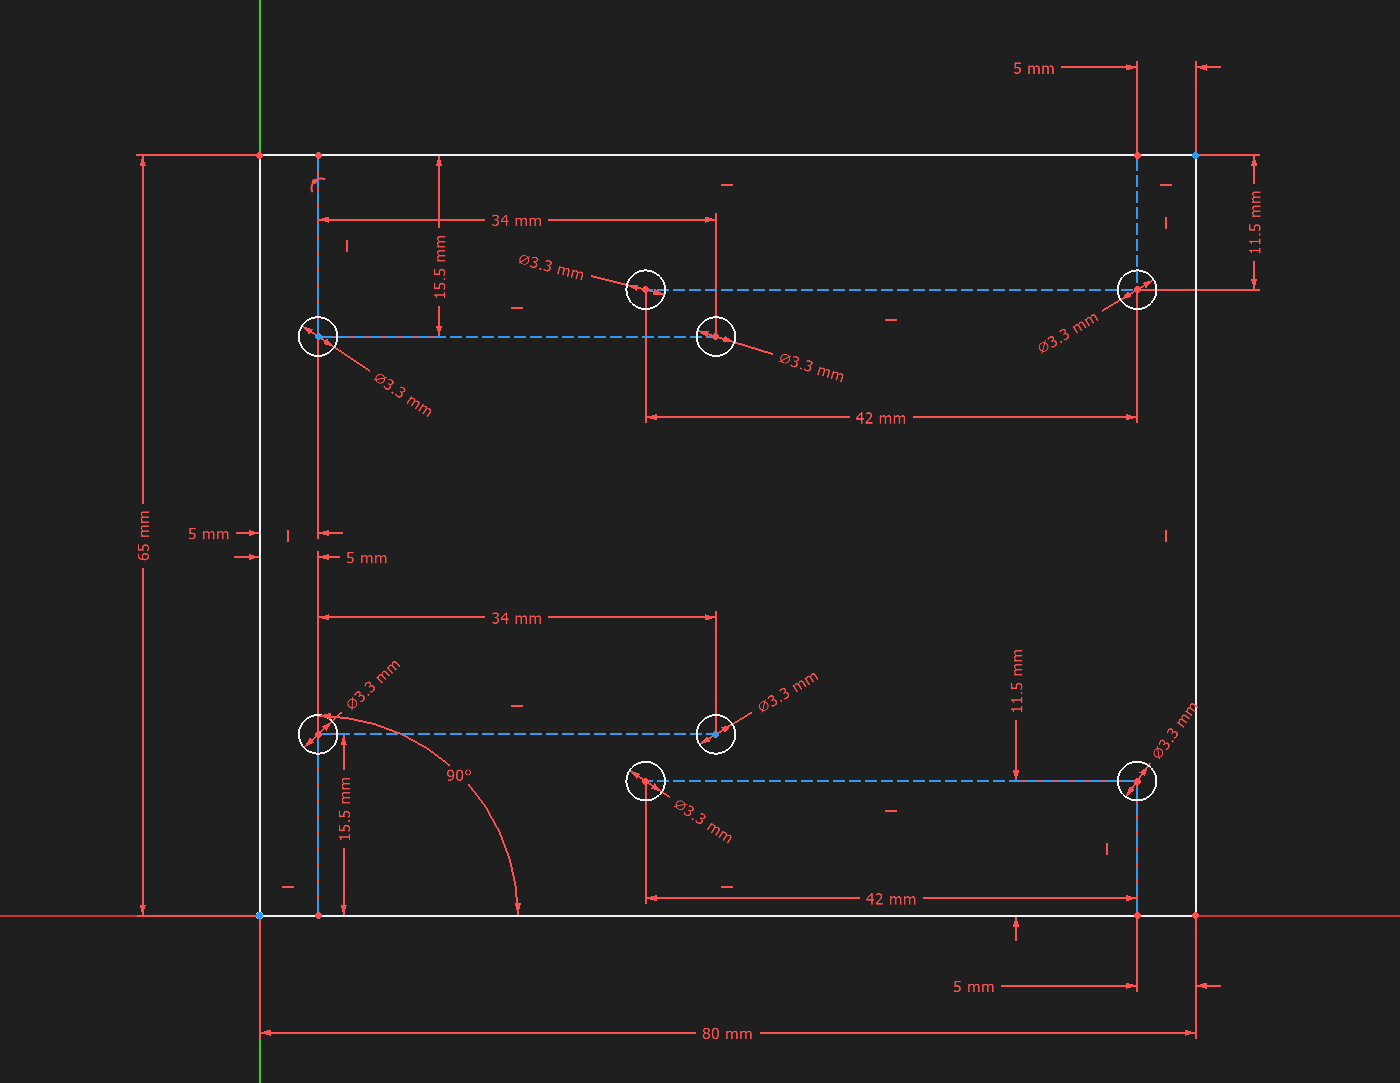
\includegraphics[width=\textwidth]{figures/lidar_mount_sketch.png}
    \caption{Sketch with dimensions in mm.}
  \end{subfigure}\hfill
  \begin{subfigure}[b]{0.40\textwidth}
    \centering
    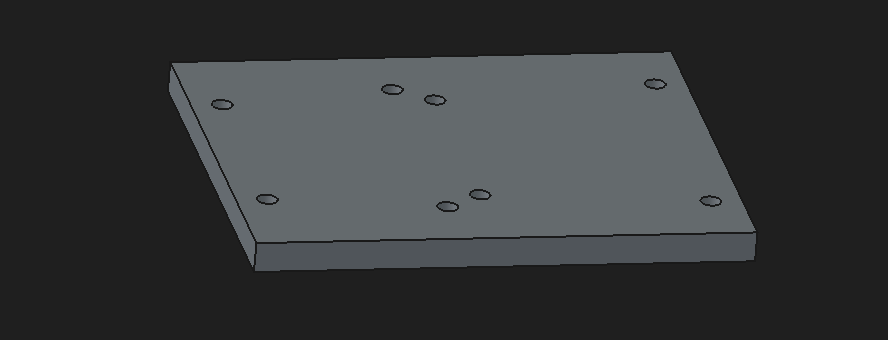
\includegraphics[width=\textwidth]{figures/lidar_mount_3d.png}
    \caption{3D model.}
  \end{subfigure}
  \caption{Adapter plate for the lidar (FreeCAD).}
  \label{fig:mount}
\end{figure}

\paragraph{Position of the lidar.} The position of the lidar relative to \texttt{base\_link} (centre between the wheels on floor level) was measured with a ruler. The centre of the lidar is about \SI{0.01}{\metre} in front of the centre of the robot and in the middle between left and right. The scan plane is about \SI{0.19}{\metre} above the floor. The orientation was checked with the hand test: a hand in front of the robot appeared on the negative $x$-axis of the \texttt{laser} frame, so the lidar is mounted turned by \SI{180}{\degree}. The transform \texttt{base\_link}~$\rightarrow$~\texttt{laser} was therefore set to $(x, y, z) = (0.01, 0, 0.19)\,\si{\metre}$ and yaw $= \pi$.

\section{Mapping and navigation}
\label{sec:slam_method}

\paragraph{Robot description and launch file.} The fixed transforms of the robot were described in a URDF file with the frames \texttt{base\_link}, \texttt{laser} and \texttt{imu\_link} (Appendix~\ref{app:code}). To start the robot with one command, a launch file \texttt{robot.launch.py} was added to the package \texttt{rasprover\_bridge}. It starts the \texttt{robot\_state\_publisher}, the bridge node with the calibrated distance scale, the lidar driver and, if wanted, the \texttt{foxglove\_bridge}. SLAM Toolbox and Nav2 were installed as ROS2 packages. At first, they were started by hand in separate terminals of the same container. Later, a second launch file \texttt{bringup.launch.py} was written, which starts everything with one command: it starts \texttt{robot.launch.py}, then SLAM Toolbox after \SI{5}{\second} and Nav2 after \SI{15}{\second}. The delays make sure that the gyroscope calibration is finished before SLAM Toolbox starts and that SLAM Toolbox already provides the transform \texttt{map}~$\rightarrow$~\texttt{odom} when Nav2 starts. With the argument \texttt{nav:=false}, only the robot and SLAM Toolbox are started, e.g.\ for mapping only.

\paragraph{Nodes.} Fig.~\ref{fig:nodes} shows all nodes and how they are connected. Table~\ref{tab:nodes} explains what each node does.

\begin{figure}[H]
  \centering
  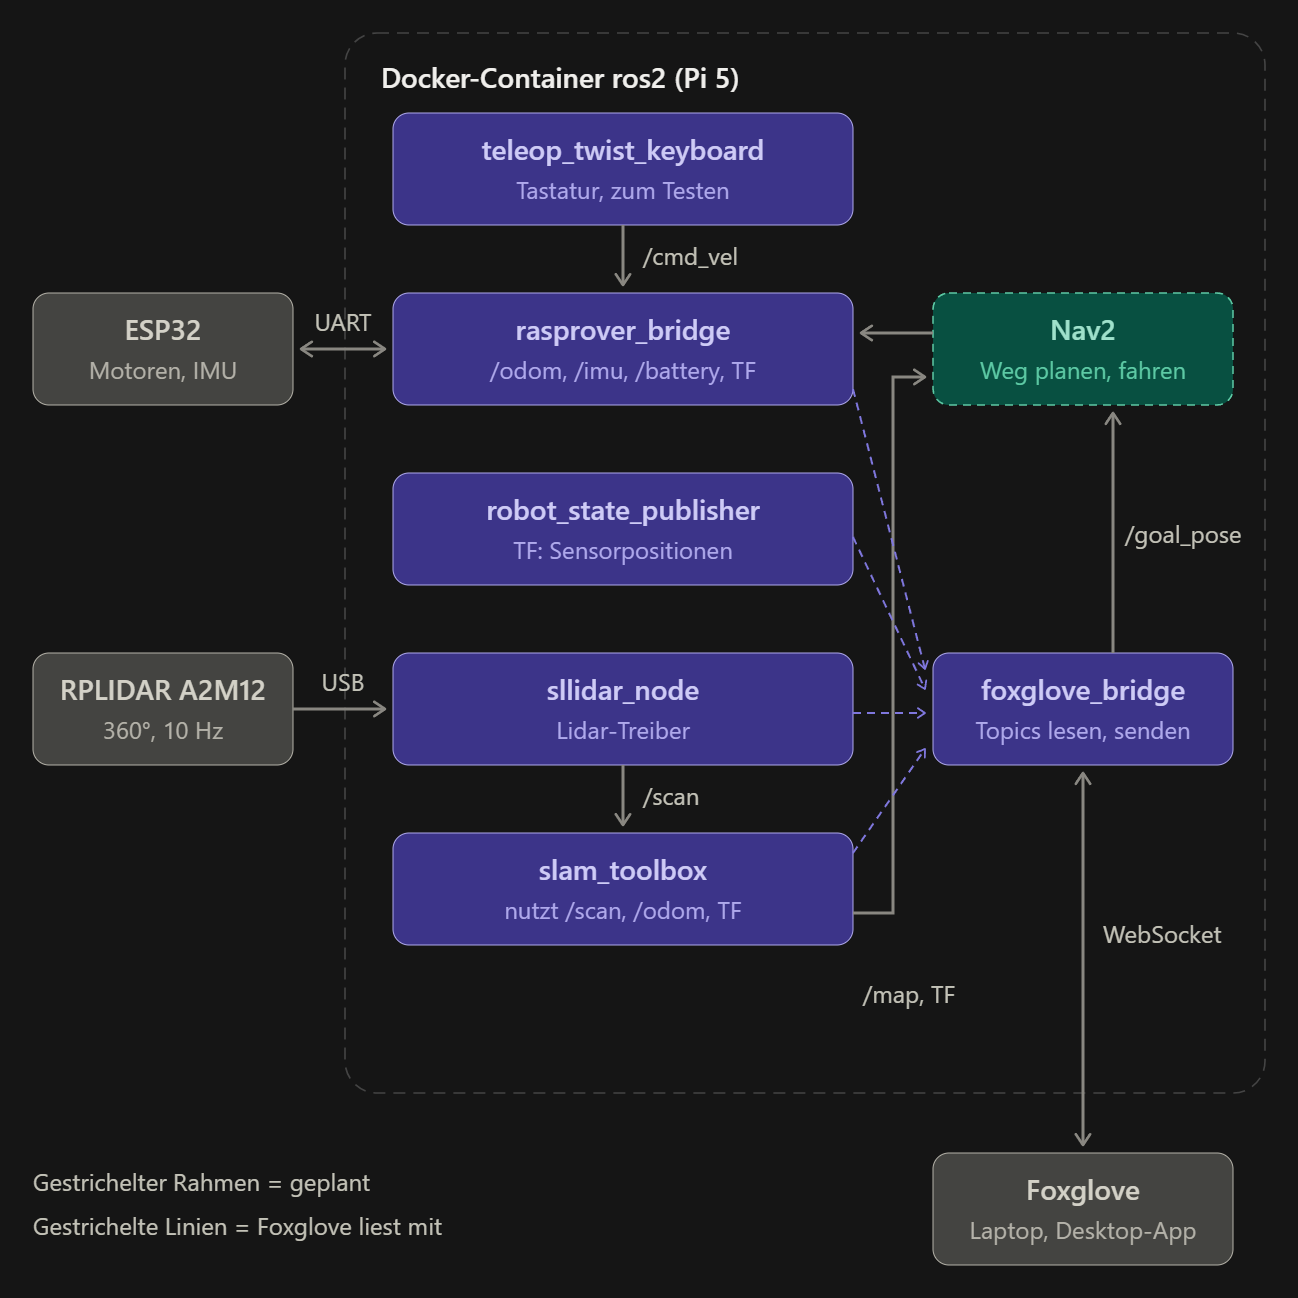
\includegraphics[width=0.85\textwidth]{figures/node_overview.png}
  \caption{Nodes and topics on the robot. \todo{Placeholder, figure will be redrawn.}}
  \label{fig:nodes}
\end{figure}

\begin{table}[H]
  \centering
  \small
  \caption{Nodes used in this work and their function.}
  \label{tab:nodes}
  \begin{tabularx}{\textwidth}{@{}>{\raggedright\arraybackslash}p{3.9cm} X >{\raggedright\arraybackslash}p{3.4cm}@{}}
    \toprule
    \textbf{Node} & \textbf{Function} & \textbf{Topics (in / out)} \\
    \midrule
    \texttt{teleop\_twist\_keyboard} & Drives the robot with the keyboard. Used for tests and for driving while creating the map. & out: \texttt{/cmd\_vel} \\
    \texttt{rasprover\_bridge} & Own node (Section~\ref{sec:bridge}). Sends the drive commands to the ESP32 and publishes the odometry, the IMU values and the battery voltage. & in: \texttt{/cmd\_vel} \newline out: \texttt{/odom}, \texttt{/imu/data\_raw}, \texttt{/battery\_state}, TF \texttt{odom}$\rightarrow$\texttt{base\_link} \\
    \texttt{robot\_state\_publisher} & Reads the URDF file and publishes the fixed positions of the sensors on the robot. & out: TF \texttt{base\_link}$\rightarrow$\texttt{laser}, \texttt{imu\_link} \\
    \texttt{sllidar\_node} & Driver of the lidar. Reads the measurements over USB and publishes them as laser scan. & out: \texttt{/scan} \\
    \texttt{slam\_toolbox} & Creates the map from the laser scans and the odometry and corrects the position of the robot in the map. & in: \texttt{/scan}, TF \newline out: \texttt{/map}, TF \texttt{map}$\rightarrow$\texttt{odom} \\
    Nav2 (several nodes) & Plans a path to the goal, follows it and avoids obstacles (Section~\ref{sec:theory_slam}). & in: \texttt{/goal\_pose}, \texttt{/map}, \texttt{/scan}, \texttt{/odom}, TF \newline out: \texttt{/cmd\_vel} \\
    \texttt{foxglove\_bridge} & Makes the topics available to the Foxglove application on the laptop (WebSocket, port 8765). Foxglove shows the scan, the map and the frames and can send goals. & in/out: all topics, e.g.\ out: \texttt{/goal\_pose} \\
    \bottomrule
  \end{tabularx}
\end{table}

\paragraph{Mapping.} The map was created with SLAM Toolbox in asynchronous online mode. In the configuration, the robot frame was changed from \texttt{base\_footprint} to \texttt{base\_link}, the maximum laser range was set to \SI{12}{\metre} as in the data sheet of the lidar~\citep{slamtec_a2m12}, and the map resolution was set to \SI{0.05}{\metre}. The robot was driven manually with \texttt{teleop\_twist\_keyboard} while the map was checked live in Foxglove. Afterwards, the map was saved with \texttt{map\_saver\_cli} from the package \texttt{nav2\_map\_server}.

\paragraph{Navigation.} Following a suggestion of the supervisor, the robot should be able to navigate and avoid obstacles with only a partial map, because mapping the whole Schlosshof in advance would take a long time. Therefore, Nav2 was started with \texttt{navigation\_launch.py} while SLAM Toolbox was running. In this setup, SLAM Toolbox provides both the map and the position of the robot, as described in the Nav2 documentation~\citep{nav2_slam}. Because the map grows while the robot drives, the planner was allowed to plan through unknown areas (\texttt{allow\_unknown: true}). In the Nav2 configuration, the robot frame was changed to \texttt{base\_link}, and the MPPI controller was used. To save computing power on the Raspberry Pi, the number of sampled trajectories of the MPPI controller (\texttt{batch\_size}) was reduced to 1000 and its visualisation was switched off. Goals were set in Foxglove with the \emph{2D pose} tool of the 3D panel, which publishes a pose on \texttt{/goal\_pose}.

For the cost maps, the robot is described as a circle around \texttt{base\_link}. The robot is about \SI{20}{\centi\metre} long and \SI{18}{\centi\metre} wide (measured with a small buffer), which gives a radius of $\sqrt{0.10^2 + 0.09^2} \approx \SI{0.14}{\metre}$. The safety zone around obstacles (\texttt{inflation\_radius}) was reduced from \SI{0.70}{\metre} to \SI{0.30}{\metre}, because with the larger values the robot could hardly move in a small room (Section~\ref{sec:nav_results}). For the first tests, low velocity and acceleration limits were used, which were increased after the first tests (Tab.~\ref{tab:nav2}).

Because the MPPI controller turned the robot with several small forward and backward movements instead of turning on the spot, the Rotation Shim Controller of Nav2 was added in front of it. If the path points more than \SI{45}{\degree} away from the heading of the robot, it first turns the robot on the spot with a commanded angular velocity of \SI{1.6}{\radian\per\second} and then hands over to the MPPI controller. Its angular acceleration limit was first set to \SI{2.5}{\radian\per\second\squared} and then increased to \SI{10}{\radian\per\second\squared} (Section~\ref{sec:nav_results}). The shim was also set to turn the robot into the final orientation at the goal (\texttt{rotate\_to\_goal\_heading}), because the MPPI controller turned the robot back and forth at the goal.

The log of Nav2 showed that the controller could not keep its rate of \SI{20}{\hertz} on the Raspberry Pi. The controller rate was therefore reduced to \SI{10}{\hertz}. So that the MPPI controller still plans \SI{2.8}{\second} ahead, its time step (\texttt{model\_dt}) was increased from \SI{0.05}{\second} to \SI{0.1}{\second} and the number of time steps was reduced from 56 to 28. In addition, Nav2 aborted goals during slow manoeuvres around obstacles because the progress checker did not detect enough progress. Its limits were therefore relaxed from \SI{0.5}{\metre} in \SI{10}{\second} to \SI{0.25}{\metre} in \SI{20}{\second}.

\begin{table}[H]
  \centering
  \small
  \caption{Nav2 parameters in the first tests and after the adjustments.}
  \label{tab:nav2}
  \begin{tabular}{@{}lll@{}}
    \toprule
    \textbf{Parameter} & \textbf{First tests} & \textbf{Adjusted} \\
    \midrule
    Max.\ linear velocity & \SI{0.25}{\metre\per\second} & \SI{0.4}{\metre\per\second} \\
    Min.\ linear velocity (reverse) & \SI{-0.15}{\metre\per\second} & \SI{-0.15}{\metre\per\second} \\
    Max.\ angular velocity & \SI{1.2}{\radian\per\second} & \SI{1.6}{\radian\per\second} \\
    Max.\ linear acceleration / deceleration & $\pm$\SI{1.0}{\metre\per\second\squared} & $\pm$\SI{1.5}{\metre\per\second\squared} \\
    Max.\ angular acceleration / deceleration & $\pm$\SI{2.0}{\radian\per\second\squared} & $\pm$\SI{2.5}{\radian\per\second\squared} \\
    Robot radius & \SI{0.22}{\metre} & \SI{0.14}{\metre} \\
    Inflation radius & \SI{0.70}{\metre} & \SI{0.30}{\metre} \\
    Rotation Shim Controller & -- & \SI{1.6}{\radian\per\second}, \SI{10}{\radian\per\second\squared} \\
    Rotation to goal heading by shim & -- & yes \\
    Controller rate & \SI{20}{\hertz} & \SI{10}{\hertz} \\
    MPPI time step / number of steps & \SI{0.05}{\second} / 56 & \SI{0.1}{\second} / 28 \\
    Progress checker & \SI{0.5}{\metre} in \SI{10}{\second} & \SI{0.25}{\metre} in \SI{20}{\second} \\
    \bottomrule
  \end{tabular}
\end{table}

The velocity and acceleration limits were set both in the MPPI controller and in the velocity smoother. The commands for starting the system are listed in Appendix~\ref{app:commands}.

\paragraph{Exploration.} For autonomous mapping, the package \texttt{explore\_lite} (ROS2 version \texttt{m-explore-ros2}) was used~\citep{m_explore}. It is not available as a binary package for ROS2 Jazzy, so it was built from source in the container, together with its message package \texttt{explore\_lite\_msgs}. It was started with its default parameters in a separate terminal after \texttt{bringup.launch.py}, as soon as Nav2 was ready. The frontiers were shown in Foxglove on the topic \texttt{/explore/frontiers}. Because the lidar only measures in one plane, open doors were closed off with a light-coloured obstacle higher than \SI{20}{\centi\metre}, so that the robot does not leave the test area.

\section{Evaluation}
\label{sec:evaluation_method}

The final tests are carried out in the Schlosshof, as planned in the project outline. Before that, the procedure was tested indoors. \todo{Adapt to the final test plan in the Schlosshof.}

\paragraph{Exploration and map.} The robot explores the test area with \texttt{explore\_lite} until no reachable frontiers are left. The duration and the number of goals are taken from the log. To evaluate the map accuracy, distances between clearly visible points (e.g.\ walls, pillars) are measured in the saved map and compared with measurements with a measuring tape. \todo{Points and distances.}

\paragraph{Reaching goals.} In the finished map, goals are set repeatedly from the same start position. For each run, it is recorded whether the goal is reached, the time between \texttt{Begin navigating} and \texttt{Goal succeeded} in the log, the number of \texttt{Failed to make progress} messages and the distance between the robot and the goal position, measured with a measuring tape. \todo{Number of goals and repetitions.}

\paragraph{Obstacle avoidance.} To test whether the robot avoids obstacles without a complete map, the robot is first driven to a place from where it cannot see a certain part of the area. An obstacle is placed there, and a goal behind the obstacle is set. The obstacle has to be higher than \SI{20}{\centi\metre}, because the lidar only measures in one plane at \SI{0.19}{\metre} above the floor. It is observed whether the robot detects the obstacle, plans a new path around it and reaches the goal. For this, the local cost map, the planned path (\texttt{/plan}) and the scan are shown in Foxglove. \todo{Obstacles (light and dark), number of repetitions.}
